\documentclass{standalone}
\renewcommand{\familydefault}{\sfdefault}

\usepackage{etoolbox}
\usepackage{tikz}
\usetikzlibrary{matrix}
\usetikzlibrary{calc}
\usetikzlibrary {arrows.meta}
\tikzset{>=Stealth}

\begin{document}
\scalebox{2}{
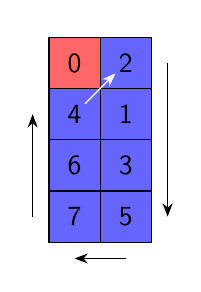
\begin{tikzpicture}[ampersand replacement=\&]
\matrix (G) at (0, 0) [matrix of nodes,
		       style={nodes={draw, minimum size=0.65cm, fill=blue!60!white}},
		       row 1 column 1/.style={nodes={draw, minimum size=0.65cm, fill=red!60!white}},
		       column sep=-\pgflinewidth,
		       row sep=-\pgflinewidth] {
	0 \& 2 \\
	4 \& 1 \\
	6 \& 3 \\
	7 \& 5 \\
};

	\draw [white, ->] ($(G-2-1.north east) - (0.2, 0.2)$) -- ($(G-1-2.south west) + (0.2, 0.2)$);
	\draw [->] ($(G-1-2.east) + (0.2, 0)$) -- ($(G-4-2.east) + (0.2, 0)$);
	\draw [->] ($(G-4-2.south) - (0, 0.2)$) -- ($(G-4-1.south) - (0, 0.2)$);
	\draw [->] ($(G-4-1.west) - (0.2, 0)$) -- ($(G-2-1.west) - (0.2, 0)$);
\end{tikzpicture}
}
\end{document}
